\documentclass[11pt,a4paper]{article}

\usepackage[margin=2.5cm]{geometry}
\usepackage[T1]{fontenc}
\usepackage{lmodern}
\usepackage{microtype}
\usepackage{graphicx}
\usepackage{booktabs}
\usepackage{tabularx}
\usepackage{array}
\usepackage{xcolor}
\usepackage{listings}
\usepackage{caption}
\usepackage{subcaption}
\usepackage{tikz}
\usetikzlibrary{arrows.meta,positioning,fit,calc,shapes.geometric,backgrounds}
\usepackage[round,authoryear]{natbib}
\usepackage[hidelinks]{hyperref}

\setlength{\parskip}{0.45em}
\setlength{\parindent}{0pt}
\renewcommand{\arraystretch}{1.15}
\newcolumntype{L}{>{\raggedright\arraybackslash}X}

% ---------------------------------------------------------------------------
% Listings
% ---------------------------------------------------------------------------
\definecolor{codebg}{RGB}{248,248,246}
\definecolor{codekw}{RGB}{0,82,147}
\definecolor{codestr}{RGB}{163,21,21}
\definecolor{codecm}{RGB}{110,110,110}

\lstdefinelanguage{TypeScript}{
  keywords={const,let,var,function,async,await,return,import,from,export,enum,interface,type,new,if,else,for,of,in,class,extends,true,false,null,undefined},
  sensitive=true,
  comment=[l]{//},
  morecomment=[s]{/*}{*/},
  morestring=[b]",
  morestring=[b]',
}
\lstdefinelanguage{json}{
  morestring=[b]",
  stringstyle=\color{codestr},
}
\lstset{
  basicstyle=\ttfamily\footnotesize,
  backgroundcolor=\color{codebg},
  keywordstyle=\color{codekw}\bfseries,
  stringstyle=\color{codestr},
  commentstyle=\color{codecm}\itshape,
  frame=single,
  rulecolor=\color{black!15},
  breaklines=true,
  columns=fullflexible,
  keepspaces=true,
  showstringspaces=false,
  numbers=left,
  numberstyle=\tiny\color{black!45},
  xleftmargin=1.5em,
  framexleftmargin=1.5em,
  aboveskip=0.6em,
  belowskip=0.6em,
}

% ---------------------------------------------------------------------------
% TikZ styles
% ---------------------------------------------------------------------------
\tikzset{
  stage/.style={draw, rounded corners=2pt, fill=blue!6, align=center, font=\footnotesize, minimum height=0.95cm, text width=2.15cm},
  llm/.style={stage, fill=orange!15},
  gate/.style={stage, fill=green!12},
  store/.style={draw, rounded corners=2pt, fill=black!5, align=center, font=\footnotesize, text width=2.3cm, minimum height=0.8cm},
  flow/.style={-{Stealth[length=2mm]}, thick},
  fb/.style={-{Stealth[length=2mm]}, thick, dashed, red!70!black},
  fn/.style={draw=blue!60, fill=blue!8, rounded corners=2pt, font=\scriptsize\ttfamily, align=center, inner sep=3pt},
  var/.style={draw=orange!70!black, fill=orange!10, rounded corners=6pt, font=\scriptsize\ttfamily, align=center, inner sep=3pt},
  cs/.style={draw=red!70!black, fill=red!8, thick, rounded corners=2pt, font=\scriptsize\ttfamily, align=center, inner sep=3pt},
  apiold/.style={draw=red!60!black, fill=red!12, rounded corners=2pt, font=\scriptsize\ttfamily, align=center, inner sep=3pt},
  apinew/.style={draw=green!50!black, fill=green!10, rounded corners=2pt, font=\scriptsize\ttfamily, align=center, inner sep=3pt},
  elabel/.style={font=\tiny\itshape, fill=white, inner sep=1pt},
}

\newcommand{\code}[1]{\texttt{#1}}
\newcommand{\morph}{\textsc{MorphAPI}}

% ---------------------------------------------------------------------------
\begin{document}

% ===========================================================================
% Title page
% ===========================================================================
\begin{titlepage}
\centering
\vspace*{1.2cm}
{\large National University of Singapore\par}
{\large School of Computing\par}
\vspace{0.4cm}
{\normalsize CP4101 B.Comp. Dissertation --- Continuous Assessment (CA) Report\par}
\vspace{1.8cm}
{\LARGE\bfseries \morph{}:\\[0.3em] Type-Grounded Hybrid AST and LLM Repair\\[0.2em] for Self-Maintaining API Migrations\par}
\vspace{1.6cm}
{\large [Your Full Name]\par}
{\normalsize Matriculation No.: [A0XXXXXX]\par}
\vspace{1.2cm}
{\normalsize Project No.: [HXXXXXX]\par}
{\normalsize Supervisor: [Supervisor Name]\par}
{\normalsize Main Evaluator: [Evaluator Name]\par}
\vfill
{\normalsize AY2026/27 Semester 1 \quad --- \quad Submitted Week 12\par}
\vspace{1.2cm}

\begin{minipage}{0.86\textwidth}
\small
\textbf{Abstract.}
Library APIs change constantly, and each breaking change forces client code to be
migrated. Rule-based codemods are precise but can only apply transformations someone
has written down; large language models (LLMs) can infer new code from vague migration
guides but invent symbols that do not exist (for example \code{CountryCode.US} where
the SDK defines \code{CountryCode.Us}). This project builds \morph{}, a hybrid
migration agent for TypeScript in which static analysis decides \emph{where} to edit and
\emph{what is true}, an LLM proposes \emph{how} to rewrite, and the TypeScript type checker
decides \emph{what is accepted}. The core artefact so far is a Code Property Graph built on
the project's real compiler program: an abstract syntax tree (AST) annotated with resolved
types, data flow, call edges and links from each deprecated API symbol to its successor.
For each call site the graph produces a compact set of \emph{slice facts} that replaces the
whole file in the prompt, and a type-checker gate rejects hallucinated names with the valid
alternatives as feedback. On a benchmark of 11 migration scenarios (21 call sites), the full
pipeline completed all 11 with gpt-4o-mini and with Claude Sonnet~4.5 and changed no
unrelated lines, whereas an LLM-only baseline completed 5 and rewrote 67\% unrelated lines.
Ablations show that the type-checker gate and one-hop impact repair account for most of
the gain. Next semester will scale the evaluation to repeated runs and real open-source
migrations.
\end{minipage}
\end{titlepage}

\tableofcontents
\newpage

% ===========================================================================
\section{Introduction and Project Objectives}
\label{sec:intro}
% ===========================================================================

\subsection{Motivation}

Software is built on third-party libraries whose APIs evolve. Parameters are renamed,
plain strings become enumerations, synchronous calls become asynchronous, results are
wrapped in pagination envelopes and authentication schemes are replaced. Empirical studies
show that breaking changes are common and that most of them are refactorings that client
developers must replicate by hand \citep{dig2006apis,xavier2017breaking}; developers
frequently delay upgrades because the migration cost is high, even when security advisories
are involved \citep{kula2018update,bogart2016break}. Migration is therefore recurring,
expensive maintenance work.

Two kinds of tools exist today. \emph{Rule-based} tools such as codemods
\citep{jscodeshift,openrewrite} operate on the abstract syntax tree (AST) and are precise,
but each transformation must be written by an engineer, and they cannot synthesise code
for conceptual changes such as a builder pattern or a JWKS key-set lookup. \emph{Generative}
tools based on large language models (LLMs) can infer such rewrites from prose migration
guides, but they hallucinate API members that look plausible and do not exist
\citep{liu2024hallucination,spracklen2025package}, rewrite unrelated code, and miss
breakage that propagates to callers.

Listing~\ref{lst:plaid} shows the running example used throughout this report. In the
old Plaid Link SDK, country codes are strings; in the new SDK they are members of an enum.
The public guide only says to ``use the country code enum for the United States''. The
value is \code{"US"}, but the member \emph{name} is \code{Us}. Without the SDK's type
declarations, an LLM writes \code{CountryCode.US}, which looks correct and does not compile.

\begin{lstlisting}[language=TypeScript, caption={Running example: a Plaid Link call that must move from \code{plaid-link-v1} (strings) to \code{plaid-link-v2} (enums).}, label={lst:plaid}]
// plaid-link-v2: enum CountryCode { Us = "US", Gb = "GB", Ca = "CA", Fr = "FR", De = "DE" }
const response = await client.linkTokenCreate({
  user: { client_user_id: userId },
  products: ["transactions"],        // v2: Products.Transactions
  country_codes: ["US"],             // v2: CountryCode.Us   (an LLM writes CountryCode.US)
  language: "en",
});
return response.link_token;
\end{lstlisting}

\subsection{Problem statement}

Given a TypeScript project that uses a deprecated API, a successor package, and an
informal migration guide, produce a minimal edit that (i) migrates every call site,
(ii) uses only symbols that exist in the successor API, (iii) repairs breakage that the
change causes in neighbouring code, and (iv) leaves unrelated code untouched.

\subsection{Objectives}

\begin{enumerate}
  \item[\textbf{O1}] \textbf{Benchmark.} Build a controlled benchmark of API-migration
        scenarios that each isolate one failure mode observed in practice (enum scaffolding,
        stale parameters, unit shifts, test evasion, payload envelopes, async contagion,
        multi-site refactoring, exception hierarchy drift, discriminator changes and
        authentication overhauls).
  \item[\textbf{O2}] \textbf{Program representation.} Design a typed program graph that
        captures what an LLM needs to know about one call site, beyond what a syntax tree
        alone provides, and reduce it to a compact prompt context.
  \item[\textbf{O3}] \textbf{Verification.} Ground the LLM's proposals in the successor
        API's real declarations, reject invented symbols and evasion, and return targeted
        feedback.
  \item[\textbf{O4}] \textbf{Impact.} Detect and repair breakage that a migration causes
        one hop away (callers, result consumers and importers).
  \item[\textbf{O5}] \textbf{Evaluation.} Compare the hybrid against an LLM-only baseline
        and against ablations that remove one mechanism at a time.
\end{enumerate}

\subsection{Scope}

The project targets TypeScript, because its compiler exposes a full type checker through a
public API \citep{tscompilerapi,bierman2014typescript} and because typed SDKs (Stripe,
Plaid, AWS, OpenAI) are widely used. ``Correct'' is judged at two levels: the type level
(the migrated program type-checks with no new diagnostics and no remaining use of the
deprecated API) and, in the per-scenario baselines, a behavioural level (for example that
amounts were converted from dollars to cents).

% ===========================================================================
\section{Literature Review}
\label{sec:lit}
% ===========================================================================

This review is organised around the three questions the project must answer: how API
migration has been automated, how programs can be represented for analysis and for
learning, and how LLM code generation can be grounded and verified.

\subsection{API evolution and automated migration}

\citet{dig2006apis} studied five Java libraries and found that over 80\% of the API changes
that broke clients were refactorings, which motivated tools that \emph{record and replay}
refactorings: CatchUp! \citep{henkel2005catchup} captured refactorings in the library
developer's IDE and replayed them on clients. LibSync \citep{nguyen2010libsync} learned
adaptation patterns from clients that had already migrated, representing API usages as
graphs. More recent work infers and applies type changes from version history
\citep{ketkar2022typechange}. A systematic review by \citet{lamothe2021review} notes that
most approaches need examples of the migration or a hand-written mapping, and that
conceptual changes beyond one-to-one mappings remain hard. Studies of developer behaviour
explain why tool support matters: developers react slowly to deprecation
\citep{robbes2012deprecation}, and ecosystem norms push the migration cost onto
clients \citep{bogart2016break}.

Industrial codemod frameworks \citep{jscodeshift,openrewrite} follow the same rule-based
principle. They give precise, reviewable edits, but every pattern has to be authored; a
rename recipe cannot decide that \code{"US"} should become \code{CountryCode.Us} unless an
engineer encodes that mapping.

LLM-based migration is recent. \citet{almeida2024migration} report first results for
migrating a Python library with ChatGPT: many migrations were correct, but some were
incomplete or introduced errors. \citet{nikolov2025google} describe Google's internal use of
LLMs for large code migrations, where generated changes are validated by builds and tests
and reviewed by humans. Both point to the same pattern that \morph{} adopts: generation must
be paired with automatic validation. Neither work provides the type-grounded, per-call-site
context and feedback that this project studies.

\subsection{Program representations}

A syntax tree records the grammatical structure of one file. Classical program analysis
adds semantic relations on top of it. The program dependence graph \citep{ferrante1987pdg}
combines control and data dependences, and program slicing \citep{weiser1981slicing}
extracts the statements relevant to a point of interest. \citet{yamaguchi2014cpg} merged
the AST, control-flow graph and program dependence graph into one \emph{Code Property
Graph} (CPG), in which nodes and edges carry key--value properties that can be queried;
they used it to find vulnerabilities. \morph{} adapts this idea to migration: the properties
of interest are resolved types, the declaration a call resolves to, and the mapping from
deprecated to successor symbols.

Learned representations follow the same intuition that structure beyond tokens matters.
\citet{allamanis2018graphs} add data-flow edges to the AST for graph neural networks.
CodeBERT \citep{feng2020codebert} pre-trains a transformer on code and text, and
GraphCodeBERT \citep{guo2021graphcodebert} adds a data-flow graph to pre-training through a
graph-guided attention mask. These models produce embeddings that measure similarity; they
do not decide whether a symbol exists in a given SDK version, which is the question a
migration gate must answer exactly (Section~\ref{sec:alternatives}).

\subsection{LLMs for code: capabilities and hallucination}

Code LLMs such as Codex \citep{chen2021codex} solve many function-level tasks, but
repository-level tasks remain hard: on SWE-bench \citep{jimenez2024swebench}, models must
edit real repositories and pass tests, and early systems resolved only a small fraction of
issues. A recurring failure is hallucination. \citet{liu2024hallucination} build a taxonomy of
hallucinations in generated code, including references to non-existent APIs and members;
\citet{spracklen2025package} show that code LLMs frequently recommend packages that do not
exist. API migration is particularly exposed: the model's training data mixes old and new
API versions, and migration guides are often vague.

\subsection{Grounding and verifying LLM output}

Three families of techniques reduce these errors.
\emph{Retrieval} puts relevant context into the prompt: retrieval-augmented generation
\citep{lewis2020rag} and repository-level retrieval such as RepoCoder
\citep{zhang2023repocoder}. Retrieval selects text by similarity; it does not guarantee
the facts are complete or type-correct.
\emph{Constrained decoding} uses static analysis during generation. Monitor-guided decoding
\citep{agrawal2023monitor} queries a language server to restrict tokens to members that exist;
Repilot \citep{wei2023repilot} uses a completion engine to prune infeasible tokens during
program repair; and type-constrained decoding \citep{mundler2025typeconstrained} enforces
well-typedness during generation. These methods require control over the decoding loop,
which hosted APIs do not expose.
\emph{Post-hoc checking and feedback} validates complete outputs. Jigsaw
\citep{jain2022jigsaw} post-processes LLM output with program analysis and repair;
Self-Debugging \citep{chen2024selfdebug} and Reflexion \citep{shinn2023reflexion} feed
execution or error messages back to the model.

\subsection{Gap and positioning}

Rule-based migration is precise but cannot synthesise; LLM migration synthesises but is not
grounded; retrieval provides context but not guarantees; constrained decoding provides
guarantees but needs access to the decoder. \morph{} combines the strengths that work with
any hosted model: (i) a typed program graph, in the spirit of code property graphs, that
produces \emph{verified} facts for one call site rather than retrieved text; (ii) a post-hoc
gate driven by the real type checker that turns compiler diagnostics into a list of valid
alternatives; and (iii) one-hop impact analysis that repairs breakage around the edit. To my
knowledge, no prior migration tool combines per-call-site typed slices, compiler-grounded
valid-option feedback and impact repair, and evaluates each through ablation.

% ===========================================================================
\section{Progress So Far}
\label{sec:progress}
% ===========================================================================

\subsection{Overview}

The implementation is a TypeScript monorepo: a core library (\code{@morphapi/core},
about 6{,}700 lines; the generic pipeline and graph modules account for about 3{,}500),
eleven pairs of old/new SDK packages with client fixtures, per-scenario baselines, and a
browser demo used for supervision meetings. Work proceeded in two phases.

\textbf{Phase 1 (per-scenario hybrid baselines).} Each scenario had a hand-written AST
finder, a hand-written oracle (a JSON allow-list of SDK symbols with known phantom
symbols), an inspector and a scenario-specific gate (behavioural, completeness, security or
anti-cheat). This established the failure taxonomy and showed that constraining the LLM to
AST spans and checking it against an oracle works: on the latest snapshot the LLM-only
baselines passed 1 of 11 scenario gates and the hybrid baselines passed 11 of 11.

\textbf{Phase 2 (generic pipeline).} Phase~1 did not scale: every new library required a
new finder, oracle and gate. Phase~2 replaced all scenario-specific code with one pipeline
(Figure~\ref{fig:pipeline}) in which a scenario is described only by its \code{tsconfig},
the deprecated symbol, the successor module and the prose guide. The rest of this section
describes Phase~2.

\begin{figure}[t]
\centering
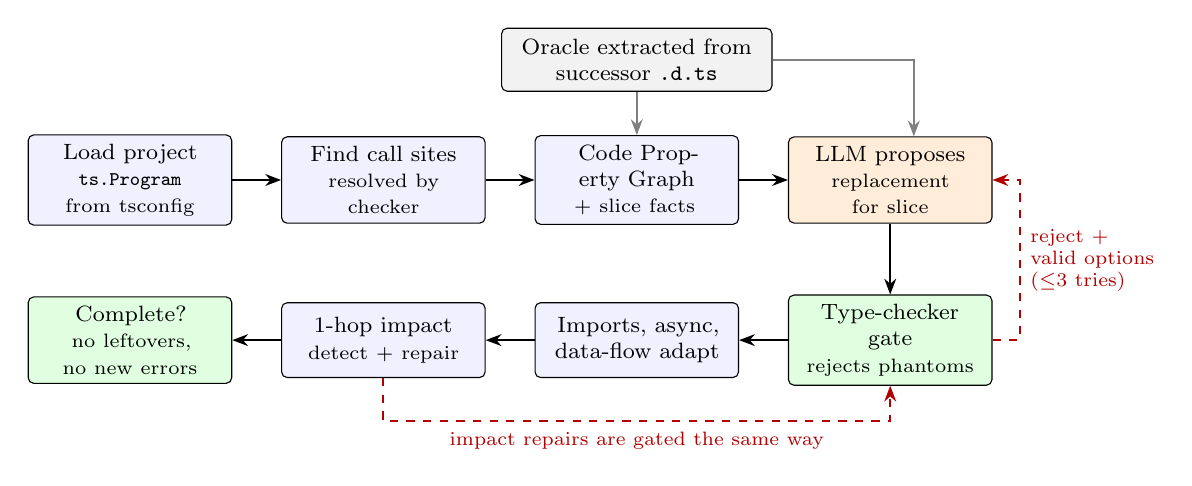
\begin{tikzpicture}[node distance=0.35cm and 0.62cm, stage/.append style={text width=2.35cm}]
  \node[stage] (load) {Load project\\\scriptsize\code{ts.Program} from tsconfig};
  \node[stage, right=of load] (find) {Find call sites\\\scriptsize resolved by checker};
  \node[stage, right=of find] (cpg) {Code Property Graph\\\scriptsize + slice facts};
  \node[llm, right=of cpg] (llm) {LLM proposes\\\scriptsize replacement for slice};
  \node[gate, below=0.9cm of llm] (gate) {Type-checker\\gate\\\scriptsize rejects phantoms};
  \node[stage, left=of gate] (post) {Imports, async,\\data-flow adapt};
  \node[stage, left=of post] (impact) {1-hop impact\\\scriptsize detect + repair};
  \node[gate, left=of impact] (done) {Complete?\\\scriptsize no leftovers, no new errors};
  \node[store, above=0.55cm of cpg, text width=3.2cm] (oracle) {Oracle extracted from\\successor \code{.d.ts}};

  \draw[flow] (load) -- (find);
  \draw[flow] (find) -- (cpg);
  \draw[flow] (cpg) -- (llm);
  \draw[flow] (llm) -- (gate);
  \draw[fb] (gate.east) -- ++(0.35,0) |- node[pos=0.25, right, font=\scriptsize, align=left]{reject +\\valid options\\($\le$3 tries)} (llm.east);
  \draw[flow] (gate) -- (post);
  \draw[flow] (post) -- (impact);
  \draw[flow] (impact) -- (done);
  \draw[flow, black!50] (oracle) -- (cpg);
  \draw[flow, black!50] (oracle.east) -| ($(llm.north)+(0.3,0)$);
  \draw[fb] (impact.south) -- ++(0,-0.55) -| node[pos=0.25, below, font=\scriptsize]{impact repairs are gated the same way} (gate.south);
\end{tikzpicture}
\caption{The generic \morph{} pipeline. Blue stages are deterministic static analysis, orange
is the LLM, green stages are judged by the TypeScript type checker. Accepted proposals
continue to the bottom row; dashed arrows are feedback loops.}
\label{fig:pipeline}
\end{figure}

\subsection{Benchmark (O1)}

Table~\ref{tab:scenarios} lists the 11 scenarios. Ten follow published failure modes of
real SDK changes; the Plaid enums mirror the published Plaid TypeScript SDK, while the others
use synthetic SDK packages that reproduce the same class of change in a controlled way. Each
scenario has an intentionally vague migration guide, the same gap that causes hallucination
in practice. In total there are 21 call sites.

\begin{table}[t]
\centering
\small
\caption{Benchmark scenarios. ``Sites'' is the number of call sites the pipeline must migrate.}
\label{tab:scenarios}
\footnotesize
\begin{tabularx}{\textwidth}{@{}l >{\raggedright\arraybackslash}p{5.6cm} L c@{}}
\toprule
ID & Deprecated API $\rightarrow$ successor & What goes wrong without grounding & Sites\\
\midrule
morphpay      & \code{ChargesApi.create} $\rightarrow$ builder           & Invented \code{CaptureMode.Automatic} & 2\\
plaid         & string codes $\rightarrow$ \code{CountryCode} enum         & \code{CountryCode.US} instead of \code{Us} & 2\\
openai        & \code{ChatCompletion.create(engine)} $\rightarrow$ \code{chat.completions.create(model)} & Stale \code{engine}, wrong client constructor & 2\\
stripe        & dollars $\rightarrow$ cents                                & Type-checks, wrong amount (behavioural) & 2\\
auth          & \code{jwt.verify(secret)} $\rightarrow$ JWKS               & \code{@ts-ignore} / \code{as any} evasion & 2\\
envelope      & \code{User[]} $\rightarrow$ \code{\{ data: User[] \}}       & Result consumers read the wrong shape & 1\\
async         & \code{S3.getObject} (sync) $\rightarrow$ \code{send(Command)} & Callers miss \code{await} & 2\\
mail          & \code{sendEmail} in several files $\rightarrow$ \code{send} & Some sites left on the old API & 4\\
stripe-errors & \code{charges.create} + \code{CardError} $\rightarrow$ new hierarchy & Stale \code{catch} of removed class & 2\\
discriminator & \code{type} $\rightarrow$ \code{event\_type} with new values & \code{switch} arms on old values & 1\\
hmac          & static token $\rightarrow$ HMAC verification               & Insecure compare kept (behavioural) & 1\\
\bottomrule
\end{tabularx}
\end{table}

\subsection{Loading the project and finding call sites}

\morph{} parses the project's \code{tsconfig.json} exactly as \code{tsc} does, so path
aliases, module resolution and installed type declarations are honoured, and builds an
incremental program session. Proposals are spliced into this session in memory and
re-checked without writing to disk; unchanged files and their diagnostics are reused.

Call sites are found \emph{by meaning, not by name}. The deprecated API is given as a
specification such as \code{plaid-link-v1\#PlaidApi.linkTokenCreate}; \morph{} resolves it
to a declaration through the checker and returns every call whose callee resolves to that
declaration, following renamed imports, namespace imports, path aliases and NodeNext
\code{.js} imports. A textual match on \code{linkTokenCreate} would miss
\code{import \{ linkTokenCreate as mk \}} and would wrongly flag an unrelated function
with the same name. On the benchmark, the generic finder agrees with the Phase~1 hand
finders on 8 of 11 scenarios; the other three hand finders target non-call sites (a
\code{catch} clause, a \code{switch} and an inline token comparison).

\subsection{The Code Property Graph: an AST with metadata (O2)}
\label{sec:cpg}

\paragraph{Why a syntax tree is not enough.}
A TypeScript AST is produced by the parser from the text of one file. It records node
kinds and positions, for example that \code{CountryCode.US} is a
\code{PropertyAccessExpression}, but nothing about meaning. To make this concrete I parsed a
snippet containing \code{enum CountryCode \{ Us = "US" \}} and \code{CountryCode.US}: the
parser reported \emph{zero} syntax errors, while the type checker reported
``\textit{Property `US' does not exist on type `typeof CountryCode'. Did you mean `Us'?}''.
Everything a migration needs to know (which library a call belongs to, what type a value has,
where it comes from, who uses the result and what replaces the old API) lives in the type
checker and in analyses built on top of it. \morph{}'s graph is the AST plus these answers.

\paragraph{Construction.}
\code{buildCodePropertyGraph} takes the program session, the project files, the call-site
spans, the deprecated symbols and the successor module, and proceeds in six steps:
\begin{enumerate}
  \item \textbf{Program.} Reuse the session's program and checker; if the successor
        package's declaration file is not yet in the program, add it so successor symbols
        can be resolved.
  \item \textbf{Functions.} Create a \code{function} node for each function declaration,
        method and arrow function bound to a constant, with \code{async}, parameter list and
        return type from the checker.
  \item \textbf{Typed data flow.} Within each function, record every occurrence of a local
        or parameter as a \code{variable} node with a role (\code{param}, \code{def},
        \code{assign}, \code{use}) and its checker type. A \code{comesFrom} edge links each
        use to the most recent definition of the same symbol; a \code{computedFrom} edge
        links a definition to the variables its initialiser reads.
  \item \textbf{Calls.} For every call expression, resolve the callee through aliases to its
        declaration; if that declaration is a project function, add a \code{calls} edge
        from the enclosing function (annotated with the line and whether it is awaited).
  \item \textbf{Successor symbols.} Look up each successor name in the successor module's
        exports through the checker and create an \code{api\_symbol} node with its printed
        type or signature.
  \item \textbf{Call sites.} For each span, find the target call, resolve its callee to the
        deprecated declaration (\code{resolves\_to}), link that declaration to every successor
        (\code{migrates\_to}), record the resolved signature, map each argument to the
        parameter it fills with both types, record why it is deprecated (an
        \code{@deprecated} JSDoc tag, the scenario's list, or the finder match), and find the
        variable the result is bound to and every later use of the \emph{same symbol}.
\end{enumerate}

Tables~\ref{tab:nodes} and~\ref{tab:edges} summarise the node and edge kinds and where each
property comes from.

\begin{table}[t]
\centering
\small
\caption{Node kinds and their metadata. Every property is produced by the TypeScript checker or by an analysis over its answers.}
\label{tab:nodes}
\begin{tabularx}{\textwidth}{@{}l L L@{}}
\toprule
Node & Properties (metadata) & Source of the metadata\\
\midrule
\code{function}   & name, async, parameters with types, return type & declaration + \code{getSignatureFromDeclaration}\\
\code{variable}   & name, role (param/def/assign/use), resolved type, line & occurrence analysis + \code{getTypeAtLocation}\\
\code{call\_site} & text, resolved signature, arguments mapped to parameters with types, deprecation reason & \code{getResolvedSignature}, \code{getTypeOfSymbolAtLocation}, JSDoc tags\\
\code{api\_symbol}& owning package, role (deprecated/successor), signature, declaration file, resolved flag & \code{getSymbolAtLocation} + alias resolution; successor module exports\\
\bottomrule
\end{tabularx}
\end{table}

\begin{table}[t]
\centering
\small
\caption{Edge kinds.}
\label{tab:edges}
\begin{tabularx}{\textwidth}{@{}l L@{}}
\toprule
Edge & Meaning\\
\midrule
\code{comesFrom}    & a use reads the value of an earlier definition of the same symbol\\
\code{computedFrom} & a definition is computed from these variable occurrences\\
\code{argument\_of} & a variable occurrence is passed into a call site (labelled with the parameter)\\
\code{contains}     & a function contains a call site\\
\code{calls}        & a function calls another project function (resolved declaration, not name)\\
\code{resolves\_to} & a call site resolves to a deprecated API symbol\\
\code{migrates\_to} & a deprecated API symbol is replaced by a successor symbol\\
\bottomrule
\end{tabularx}
\end{table}

\paragraph{Worked example.}
Figure~\ref{fig:cpg} shows the graph for the first Plaid call site (16 nodes and 15 edges in
total; the figure shows the part around the call at line~14). The checker labels
\code{client} as \code{PlaidApi} from \emph{plaid-link-v1}, which is how \morph{} knows this
call must be migrated; the data-flow edges show that \code{response} is computed from
\code{client} and \code{userId} and consumed at line~22; and the \code{migrates\_to} edges point to
the three successor symbols, including \code{CountryCode}.

\begin{figure}[t]
\centering
\resizebox{0.97\textwidth}{!}{%
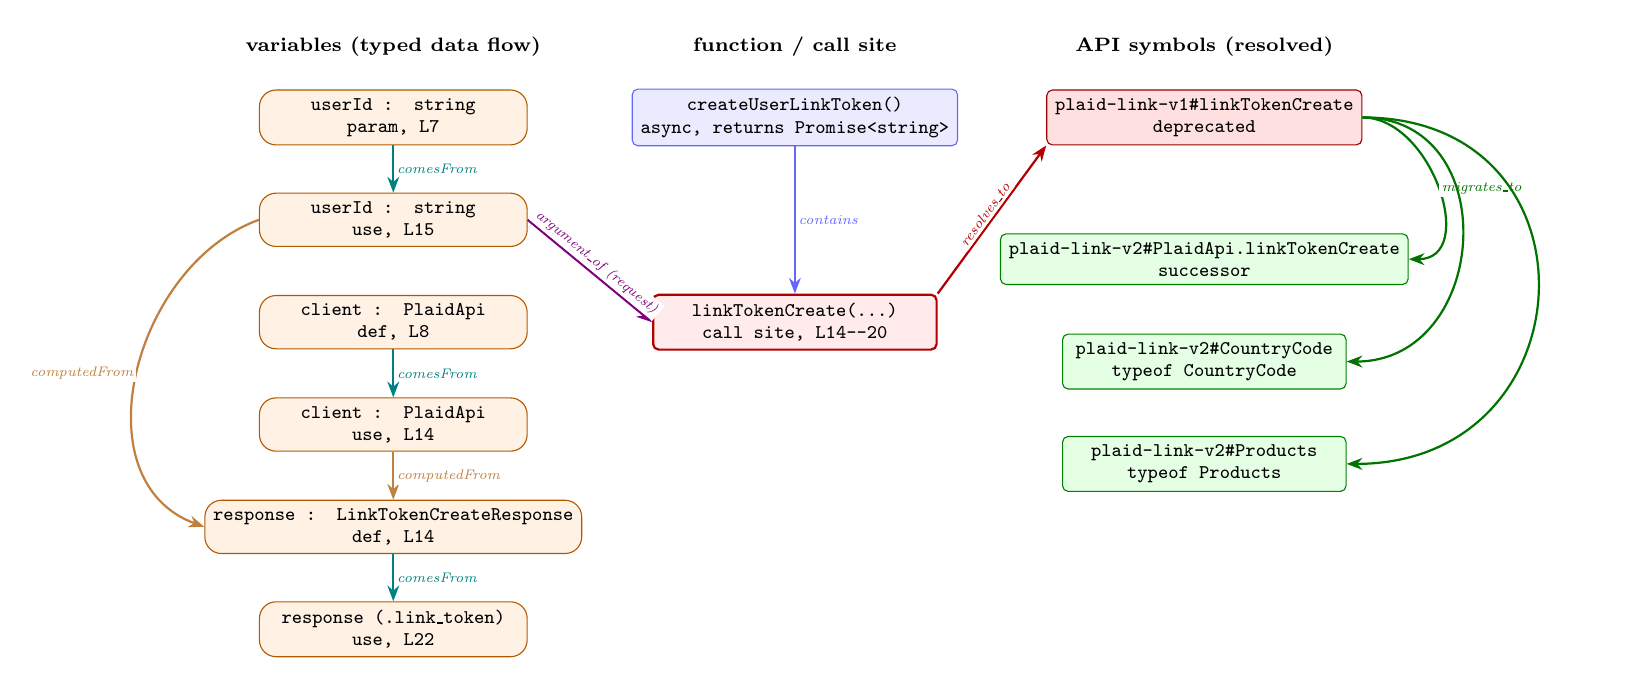
\begin{tikzpicture}[x=1cm,y=1cm]
  \node[font=\scriptsize\bfseries] at (2.5,7.3) {variables (typed data flow)};
  \node[font=\scriptsize\bfseries] at (7.6,7.3) {function / call site};
  \node[font=\scriptsize\bfseries] at (12.8,7.3) {API symbols (resolved)};

  \node[var, minimum width=3.4cm] (v0) at (2.5,6.4) {userId : string\\param, L7};
  \node[var, minimum width=3.4cm] (v3) at (2.5,5.1) {userId : string\\use, L15};
  \node[var, minimum width=3.4cm] (v1) at (2.5,3.8) {client : PlaidApi\\def, L8};
  \node[var, minimum width=3.4cm] (v2) at (2.5,2.5) {client : PlaidApi\\use, L14};
  \node[var, minimum width=3.4cm] (v4) at (2.5,1.2) {response : LinkTokenCreateResponse\\def, L14};
  \node[var, minimum width=3.4cm] (v5) at (2.5,-0.1) {response (.link\_token)\\use, L22};

  \node[fn, minimum width=3.6cm] (f) at (7.6,6.4) {createUserLinkToken()\\async, returns Promise<string>};
  \node[cs, minimum width=3.6cm] (cs) at (7.6,3.8) {linkTokenCreate(\dots)\\call site, L14--20};

  \node[apiold, minimum width=3.6cm] (old) at (12.8,6.4) {plaid-link-v1\#linkTokenCreate\\deprecated};
  \node[apinew, minimum width=3.6cm] (n1) at (12.8,4.6) {plaid-link-v2\#PlaidApi.linkTokenCreate\\successor};
  \node[apinew, minimum width=3.6cm] (n2) at (12.8,3.3) {plaid-link-v2\#CountryCode\\typeof CountryCode};
  \node[apinew, minimum width=3.6cm] (n3) at (12.8,2.0) {plaid-link-v2\#Products\\typeof Products};

  \draw[flow, teal] (v0) -- node[elabel, right]{comesFrom} (v3);
  \draw[flow, teal] (v1) -- node[elabel, right]{comesFrom} (v2);
  \draw[flow, brown] (v2) -- node[elabel, right]{computedFrom} (v4);
  \draw[flow, brown] (v3.west) to[out=200, in=160, looseness=1.1] node[elabel, left]{computedFrom} (v4.west);
  \draw[flow, teal] (v4) -- node[elabel, right]{comesFrom} (v5);

  \draw[flow, blue!60] (f) -- node[elabel, right]{contains} (cs);
  \draw[flow, violet] (v3.east) -- node[elabel, above, sloped]{argument\_of (request)} (cs.west);
  \draw[flow, red!70!black] (cs.north east) -- node[elabel, above, sloped]{resolves\_to} (old.south west);
  \draw[flow, green!45!black] (old.east) to[out=0, in=0, looseness=1.2] node[elabel, right]{migrates\_to} (n1.east);
  \draw[flow, green!45!black] (old.east) to[out=0, in=0, looseness=1.5] (n2.east);
  \draw[flow, green!45!black] (old.east) to[out=0, in=0, looseness=1.8] (n3.east);
\end{tikzpicture}}
\caption{Part of the Code Property Graph for the Plaid call at line 14. The call site also
carries its resolved signature, \code{(request: LinkTokenCreateRequest) =>
Promise<LinkTokenCreateResponse>}. Every type label and every arrow to an API symbol comes
from the TypeScript checker; a plain AST contains only the node kinds and positions.}
\label{fig:cpg}
\end{figure}

\paragraph{What the graph adds over a plain AST.}
Table~\ref{tab:astvscpg} summarises the difference on the running example. The plain AST
can locate the call and give its text; every other row needs the checker.

\begin{table}[t]
\centering
\small
\caption{Plain AST versus \morph{}'s Code Property Graph on the Plaid call.}
\label{tab:astvscpg}
\begin{tabularx}{\textwidth}{@{}L L L@{}}
\toprule
Question & Plain AST & Code Property Graph\\
\midrule
What is \code{client}? & an identifier & \code{PlaidApi} from plaid-link-v1\\
Is this call the deprecated API? & name match only; misses aliases & resolved declaration in plaid-link-v1\\
What replaces it? & --- & \code{PlaidApi.linkTokenCreate}, \code{CountryCode}, \code{Products} with types\\
Where does \code{userId} come from? & --- & parameter of \code{createUserLinkToken}, line 7, \code{string}\\
Who uses the result? & unrelated identifier nodes & \code{response.link\_token} at line 22 (same symbol)\\
Who calls this function? & --- & \code{calls} edges, with awaited/not awaited\\
Is \code{CountryCode.US} valid? & yes (valid grammar) & no; members are \code{Us}, \code{Gb}, \code{Ca}, \code{Fr}, \code{De}\\
Is \code{PLAID\_SECRET} always defined? & --- & \code{string | undefined}; successor requires \code{string}\\
\bottomrule
\end{tabularx}
\end{table}

\paragraph{Graph health.}
Because a mis-configured project silently degrades types to \code{any}, the graph reports
its own health: the fraction of checked calls whose callee is unresolved or collapsed to
\code{any}, project files missing from the program, and \code{tsconfig} errors. Explicit
\code{any} written by the developer is listed separately. A headless check
(\code{npm run graph:cli}) fails if any file is missing or the collapse rate is above 0\%;
all 11 scenarios currently pass (Plaid: 0 of 8 unresolved).

\subsection{Slice facts: what the LLM receives}

For each call site, \code{sliceFactsFor} builds the graph focused on that site and reads a
fixed set of facts off it (Listing~\ref{lst:facts}). The prompt contains the \emph{slice}
(the call and its member chain, or the enclosing statement for builder and multi-step
successors), these facts, the successor API surface and the guide; it never contains the
whole file.

\begin{lstlisting}[language=json, caption={Slice facts for the Plaid call at line 14 (abridged).}, label={lst:facts}, numbers=none]
{ "target_call": "client.linkTokenCreate({ ..., country_codes: [\"US\"], ... })",
  "slice": { "file": "link.ts", "lines": [14, 20] },
  "resolved_api": { "symbol": "plaid-link-v1#linkTokenCreate", "deprecated": true,
    "signature": "(request: LinkTokenCreateRequest): Promise<LinkTokenCreateResponse>" },
  "successor_api": [ { "symbol": "plaid-link-v2#PlaidApi.linkTokenCreate" },
                     { "symbol": "plaid-link-v2#CountryCode", "signature": "typeof CountryCode" },
                     { "symbol": "plaid-link-v2#Products",    "signature": "typeof Products" } ],
  "arguments": [ { "index": 0, "param": "request", "paramType": "LinkTokenCreateRequest" } ],
  "data_flow": [ { "variable": "userId", "declared_type": "string",
                   "origin": "parameter of createUserLinkToken() (line 7)" } ],
  "result": { "binding": "response", "type": "LinkTokenCreateResponse",
              "downstream_usages": ["response.link_token at line 22"] },
  "enclosing_function": { "name": "createUserLinkToken", "async": true,
                          "return_type": "Promise<string>" },
  "callers_1hop": [] }
\end{lstlisting}

Each field is a graph query: \code{resolved\_api} follows \code{resolves\_to};
\code{successor\_api} follows \code{migrates\_to}; \code{data\_flow} follows
\code{argument\_of} into the site and then \code{comesFrom} back to the definition, whose
declaration the checker classifies as a parameter, local or import; \code{result} walks up
from the call to its binding and collects later identifiers that resolve to the same symbol;
\code{callers\_1hop} reads the \code{calls} edges into the enclosing function.

\paragraph{Token cost.}
The facts are not smaller than the file on these fixtures (Plaid: file 259 tokens, slice 44,
facts 505), because they add information the file does not state. The benefit claimed is
precision and locality, not token savings; Section~\ref{sec:eval} measures it.

\subsection{Oracle extraction and the type-checker gate (O3)}

\paragraph{Oracle.}
Phase~1 used hand-written JSON oracles. Phase~2 extracts the oracle from the successor
package's declaration file: \code{extractOracle} lists the module's exports through the
checker, collects members of reachable types (following return types of methods and
factories), and records how to obtain a value of each type (constructor or factory
signature). For Plaid it finds 7 exports, including \code{createPlaidClient}, \code{CountryCode},
\code{Products} and \code{PlaidApi} (whose member is \code{linkTokenCreate}), and that a
\code{PlaidApi} is obtained by calling \code{createPlaidClient(\{ clientId, secret \})}.
The oracle feeds the prompt, import reconciliation and the gate's suggestions.

\paragraph{Gate.}
A proposal is spliced into the in-memory program and only diagnostics inside the patched
range are judged (the rest are left to impact analysis). Diagnostics are classified by
TypeScript error code: missing members (TS2339, TS2551) and missing names (TS2304, TS2552)
are \emph{phantoms}; missing modules or exports (TS2305, TS2307, TS2724) are phantoms; other
errors are type errors, and for a string or number literal the gate lists the literal members
of the expected union. For a missing member, the gate asks the checker for the properties of
the receiver's type \emph{at the error location} and ranks them by case-insensitive match and
edit distance. It also rejects evasion (\code{@ts-ignore}, \code{as any}) and leftovers (the
proposal still calls the deprecated symbol), and treats dynamic access such as
\code{obj["x"]} as a warning. Rejections are turned into feedback and the model retries, up
to three attempts; there is no template fallback.

Listing~\ref{lst:gate} shows the gate on the Plaid call from the saved gpt-4o-mini run. The
first proposal used \code{CountryCode.US}; the gate rejected it with the valid options, and
the second proposal was accepted. The same happened for \code{GB}$\rightarrow$\code{Gb}.

\begin{lstlisting}[caption={Gate feedback on the Plaid call (saved run, gpt-4o-mini).}, label={lst:gate}, numbers=none]
Attempt 1  country_codes: [CountryCode.US]
  REJECTED  phantom  TS2551  "Symbol US does not exist on typeof CountryCode."
            Valid options: [Us, Ca, De]
Attempt 2  country_codes: [CountryCode.Us]
  ACCEPTED
\end{lstlisting}

\subsection{Follow-up steps and impact repair (O4)}

After a proposal is accepted: (i) if it introduced \code{await} in a non-async function,
the function becomes \code{async} and its return type \code{Promise<\dots>}; (ii) successor
imports are added in the file's quote style and unused imports from the deprecated module are
removed; (iii) if the result type changed (for example an envelope instead of an array),
an adapter or read-path rewrite is tried and kept only if it restores the baseline diagnostics.
Then \textbf{one-hop impact} compares function signatures before and after and reports
\code{missing\_await}, \code{same\_api\_leftover}, \code{deprecated\_module\_use},
\code{stale\_import} and \code{new\_type\_error} in changed files, their callers and importers.
Missing awaits are fixed deterministically; the rest go back to the LLM as statement repairs,
gated the same way, and a repair is kept only if it reduces the file's error count (at most two
rounds). A run is \emph{complete} when every site was accepted, nothing resolves to or is
imported from the deprecated API, and there are no diagnostics beyond the baseline.

\subsection{Design alternatives investigated}
\label{sec:alternatives}

\begin{itemize}
  \item \textbf{Whole-file prompting vs.\ slices.} The LLM-only baseline gives the model the
        whole file. It is cheaper in tokens but rewrites unrelated code (Section~\ref{sec:eval}).
        Slices with facts were chosen for locality.
  \item \textbf{Hand-written oracles vs.\ extracted oracles.} Phase~1 oracles listed allowed
        symbols and known phantoms (e.g.\ \code{CountryCode.US}). They worked but had to be
        written per library and could go stale. Phase~2 reads the declarations and lets the
        checker judge, which removes per-library authoring.
  \item \textbf{Template fallback.} An early version substituted a hand-written correct answer
        when the model failed every attempt. This hid failures and was removed; a site that
        fails all attempts is now reported as not migrated.
  \item \textbf{Learned graph embeddings (GraphCodeBERT).} I prototyped a GraphCodeBERT
        \citep{guo2021graphcodebert} service that embedded functions with their data-flow graph
        and ranked code similar to a deprecated call. It found semantically similar code, but
        embeddings give similarity scores, not the yes/no answer the gate needs (``does
        \code{CountryCode.US} exist?''), and it added a Python and GPU dependency. It was set
        aside in favour of the type checker; it may return for finding non-call sites that do
        not mention the deprecated API (Section~\ref{sec:plan}).
  \item \textbf{Pure AST recipes.} Four scenarios have hand-written AST-only pilots. They
        migrate what the recipe enumerates and stop: e.g.\ in \emph{async} the leaf is migrated
        but the caller's missing \code{await} is detected and left unfixed; in \emph{mail} two
        of four sites remain. This confirms the expected ceiling of rule-based migration.
\end{itemize}

\subsection{Preliminary evaluation (O5)}
\label{sec:eval}

\paragraph{Setup.}
All arms run the same code path with mechanisms switched off: \textbf{LLM-only} (whole file,
one rewrite, no gate, no impact); \textbf{No slices} (whole file instead of slice facts, with
gate and impact); \textbf{No gate} (gate findings recorded but never rejected, one attempt);
\textbf{No impact} (no impact repair). The model is gpt-4o-mini at temperature 0.2; the full
pipeline was also run with Claude Sonnet~4.5. ``Churn'' is the share of changed lines that
belong to no migrated site, impact repair, import or deterministic follow-up.

\begin{table}[t]
\centering
\small
\caption{Pipeline results on 11 scenarios / 21 call sites (one run per arm; gpt-4o-mini unless stated).}
\label{tab:results}
\footnotesize
\begin{tabularx}{\textwidth}{@{}l c c c r L@{}}
\toprule
Arm & Complete & \shortstack{Phantoms\\rejected} & Churn & \shortstack{Prompt\\tokens} & Incomplete scenarios\\
\midrule
\textbf{MorphAPI (all)}         & \textbf{11/11} & 10 & \textbf{0\%} & 43{,}321 & ---\\
MorphAPI, Claude Sonnet 4.5     & 11/11 & 4  & 0\%  & 41{,}637 & ---\\
LLM-only (whole file)           & 5/11  & -- & 67\% & 6{,}267  & morphpay, plaid, auth, envelope, mail, discriminator\\
No slices (file + gate + impact)& 10/11 & 12 & 0\%  & 42{,}049 & stripe-errors\\
No gate / feedback              & 7/11  & -- & 0\%  & 40{,}894 & async, morphpay, openai, stripe-errors\\
No impact repair                & 6/11  & 9  & 0\%  & 34{,}812 & discriminator, mail, morphpay, openai, stripe-errors\\
\bottomrule
\end{tabularx}
\end{table}

\paragraph{Results.}
Table~\ref{tab:results} summarises the runs. The full pipeline completed all 11 scenarios
with both models and changed no unrelated lines; the gpt-4o-mini result was the same on
three consecutive full runs. The LLM-only baseline completed 5, and 155 of its 232 changed
lines (67\%) were unrelated to the migration. On Plaid it produced \code{CountryCode.US} and
\code{CountryCode.GB} and ended with two TS2551 errors.

\paragraph{What the ablations show.}
Removing impact repair costs the most (6/11): breakage one hop away (callers that must now
await, catch clauses on removed error classes, switch arms on old values) is never repaired.
Removing the gate costs 4 scenarios: phantoms are accepted without feedback. On Plaid, the
no-gate run still completed because impact repair, which also uses the checker, later caught
the new type error and fixed \code{US}$\rightarrow$\code{Us}; both safety nets depend on type
information. Replacing slice facts with the whole file costs only one scenario
(stripe-errors, where the model kept calling \code{paymentIntents} on the old client), so the
main value of slices here is locality rather than completion. Running the first Claude
experiment also exposed two generic weaknesses that were fixed for both models: literal
type errors now list the allowed literal values, and a stray pair of backticks around a
one-line answer (which TypeScript parses as a template string) is stripped.

\paragraph{Threats to validity.}
(i) One run per arm; LLMs are non-deterministic, so these are snapshot results, not rates.
(ii) The fixtures are small (one to three files) and mostly synthetic; results may not transfer
to large real projects. (iii) Completion is a type-level judgement: the pipeline does not yet
run the behavioural checks (e.g.\ the unit conversion in \emph{stripe}) that the Phase~1
baselines had. (iv) Impact analysis is one hop. (v) The successor symbol list per scenario is
configured, not discovered; the generic finder handles call sites only, so the inline token
comparison in \emph{hmac} is not migrated. (vi) The extracted oracle's member lists for
enums currently record string-prototype members rather than the enum members; the gate is not
affected because it queries the checker at the error location, but this should be fixed.

\subsection{Tooling for supervision}

A browser demo (\code{npm run demo:ui}) shows, for any scenario, the source with the
call site highlighted, the typed syntax tree, the typed data-flow graph, the full Code
Property Graph with clickable nodes, the slice facts with token counts, the one-hop impact
and graph health, and the pipeline run with every gate attempt and the final diff. Runs can be
replayed from saved JSON or started live, which makes the mechanism inspectable during
meetings.

% ===========================================================================
\section{Research Plan for Next Semester}
\label{sec:plan}
% ===========================================================================

\subsection{Research questions}

\begin{enumerate}
  \item[\textbf{RQ1}] How much does type-grounded context and feedback improve migration
        completeness and locality over LLM-only migration, measured over repeated runs and
        several models?
  \item[\textbf{RQ2}] Which mechanism (slice facts, type-checker gate, impact repair)
        contributes most, and does the answer change with model strength?
  \item[\textbf{RQ3}] Does the approach transfer from controlled fixtures to real migrations
        in open-source TypeScript projects?
  \item[\textbf{RQ4}] How often does a type-correct migration still change behaviour, and can
        behavioural checks be integrated into the generic pipeline?
\end{enumerate}

\subsection{Planned work}

\begin{enumerate}
  \item \textbf{Statistical evaluation.} Run every arm at least five times per scenario with
        gpt-4o-mini, Claude and one open-weight model; report completion rates with confidence
        intervals, phantom counts, attempts, churn and cost.
  \item \textbf{Real-world benchmark.} Mine 15--25 real migrations from open-source TypeScript
        repositories (for example major-version upgrades of the OpenAI, Stripe and AWS SDKs),
        use the developers' commits as references, and compare with the pipeline's output.
  \item \textbf{Behavioural gates in the pipeline.} Port the Phase~1 behavioural, security
        and completeness checks into the generic pipeline as optional test hooks, so that
        ``complete'' can also mean ``tests pass''.
  \item \textbf{Graph improvements.} Extend impact from one hop to a bounded transitive
        closure; fix enum member extraction in the oracle; discover successor symbols
        automatically from the declarations and the guide instead of configuring them; and
        reach non-call sites (catch clauses, switches, inline comparisons) through type
        relationships, possibly reusing learned embeddings for candidate ranking.
  \item \textbf{Baselines.} Add a codemod baseline (jscodeshift recipes) for the real-world
        set, and compare with a retrieval-only context (similar code from the repository
        instead of graph facts).
  \item \textbf{Write-up.} Final report, demo and presentation.
\end{enumerate}

\subsection{Timeline}

\begin{table}[h]
\centering
\small
\caption{Plan for Semester 2 (weeks of the NUS academic calendar).}
\label{tab:timeline}
\begin{tabularx}{\textwidth}{@{}l L l@{}}
\toprule
Weeks & Work & Deliverable\\
\midrule
Break       & Fix oracle enum extraction; repeated-run harness; add open-weight model & multi-seed runs on current benchmark\\
1--3        & Mine and set up real-world migrations; codemod baseline & real-world benchmark (15--25 cases)\\
4--6        & Behavioural/test hooks in pipeline; transitive impact; successor discovery & pipeline v2\\
Recess      & Full experiment matrix (arms $\times$ models $\times$ seeds $\times$ benchmarks) & results tables\\
7--9        & Analysis: RQ1--RQ4, error taxonomy of failures & draft evaluation chapter\\
10--11      & Final report writing; demo polish & full draft to supervisor\\
12--13      & Revisions, presentation & final report and presentation\\
\bottomrule
\end{tabularx}
\end{table}

\subsection{Risks}

Real projects may not compile cleanly before migration, which weakens a type-checker gate;
the pipeline already compares against baseline diagnostics, and projects that cannot build
will be excluded and reported. API costs for repeated runs are bounded by using a small model
for most runs and the larger model for a subset. If behavioural tests are unavailable for real
projects, developer commits will serve as the reference.

% ===========================================================================
\section{Conclusion}
% ===========================================================================

This semester established the problem, the benchmark and a working generic pipeline. The
main technical contribution so far is a Code Property Graph built on the real TypeScript
program, which turns a syntax tree into verified facts about one call site (types, resolved
declarations, data flow, callers, result consumers and successor symbols), together with a
type-checker gate that turns compiler diagnostics into valid-option feedback. On 11 scenarios,
the pipeline completed every migration with zero unrelated edits where an LLM-only baseline
completed five, and ablations indicate that the gate and impact repair are the critical parts.
Next semester will test whether these results hold over repeated runs, other models and real
open-source migrations.

\bibliographystyle{plainnat}
\bibliography{references}

\end{document}
